\documentclass[beamer,handout,tikz]{standalone}

\usepackage{tikz}
\usepackage{amssymb}
\usetikzlibrary{shapes.geometric,calc,decorations.markings}


	%Credit: https://tex.stackexchange.com/questions/99119/beamer-problematic-use-of-visible-and-only-in-combination-with-tikz-to-draw-a
  \tikzset{
    invisible/.style={opacity=0},
    visible on/.style={alt=#1{}{invisible}},
    alt/.code args={<#1>#2#3}{%
      \alt<#1>{\pgfkeysalso{#2}}{\pgfkeysalso{#3}} % \pgfkeysalso doesn't change the path
    },
  }

\begin{document}
	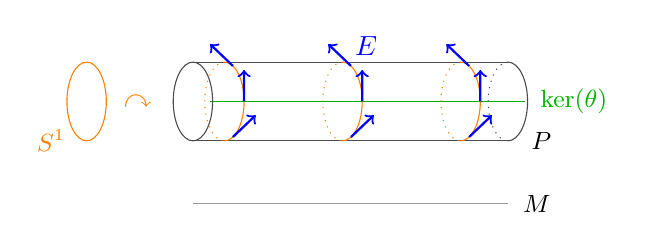
\begin{tikzpicture}[
    tangent/.style={
        decoration={
            markings,% switch on markings
            mark=
                at position #1
                with
                {
                    \coordinate (tangent point-\pgfkeysvalueof{/pgf/decoration/mark info/sequence number}) at (0pt,0pt);
                    \coordinate (tangent unit vector-\pgfkeysvalueof{/pgf/decoration/mark info/sequence number}) at (1,0pt);
                    \coordinate (tangent orthogonal unit vector-\pgfkeysvalueof{/pgf/decoration/mark info/sequence number}) at (0pt,1);
                }
        },
        postaction=decorate
    },
    use tangent/.style={
        shift=(tangent point-#1),
        x=(tangent unit vector-#1),
        y=(tangent orthogonal unit vector-#1)
    },
    use tangent/.default=1
]
		\draw[yshift=-.8cm,black!40] (0,0) -- (4,0) node[black,right=2pt] {\small $M$};
		\draw[visible on=<4->,yshift=.5cm,xshift=.22cm,green!70!black] (0,0) -- (4,0) node[green!70!black,right=2pt] {\small $\textrm{ker}(\theta)$};
		\begin{scope}[xshift=-1.35cm]
		\draw[orange] (0,.5) ellipse (.25 and .5);
		\end{scope}

		\node[orange] at (-1.8,0) {\small $S^1$};

		\node[orange] at (-.7,.5) {$\curvearrowright$};

		\draw[black!70] (0,.5) ellipse (.25 and .5);
		\draw[black!70] (4,0) arc (-90:90:.25 and .5);
		\draw[dotted,black!70] (4,1) arc (90:270:.25 and .5);
		\draw[black!70] (0,0) -- (4,0) node[black,right=5pt] {\small $P$};
		\draw[black!70] (0,1) -- (4,1);

		\foreach \x in {-1,.5,...,2}
		{
			\begin{scope}[xshift=\x cm]
				\draw[orange,xshift=1.4cm,tangent=0.1,tangent=0.5,tangent=0.9] (0,0) arc (-90:90:.25 and .5);
				\draw[orange,dotted,xshift=1.4cm] (0,1) arc (90:270:.25 and .5);

				\draw [visible on=<3->,blue,->, thick, use tangent] (0,0) -- (.4,0);
				\draw [visible on=<3->,blue,->, thick, use tangent=2] (0,0) -- (.4,0);
				\draw [visible on=<3->,blue,->, thick, use tangent=3] (0,0) -- (.4,0);
			\end{scope}

		}

		\node[visible on=<3->,blue] at (2.2,1.2) {$E$};
	\end{tikzpicture}
\end{document}